% !TEX root = ../../../main.tex

\toggletrue{image}
\toggletrue{imagehover}
\chapterimage{circumference_formula}
\chapterimagetitle{\uppercase{Circumference Formula}}
\chapterimageurl{https://xkcd.com/1184/}
\chapterimagehover{Assume r' refers to the radius of Earth Prime, and r'' means radius in inches.}

\chapter{Schlüsselvereinbarng mit \texttt{DIFFIE-HELLMAN-MERKLE}}
\label{chapter-schluesselvereinbarung-diffie-hellman-merkle}

Whitfield Diffie und Martin Hellman präsentierten 1976 die Publikation \say{New Directions in Cryptography}. Darin präsentieren Sie Ihre Lösung zur Schlüsselvereinbarung. Dieses Protokoll ist gewissermassen der Standard für die Schlüsselfestlegung. Bei der Entwicklung des Protokolls profitierten die beiden Forscher von den Arbeiten von Ralph Merkle. Dieser wird in der Publikation auch erwähnt. Deshalb ist das Protokoll heute unter dem Namen \textbf{Diffie-Hellman-Merkle-Schlüsselvereinbarung} bekannt. Das Verfahren wird manchmal auch mit DH-Schlüsselvereinbarung oder DHM-Schlüsselvereinbarung abgekürzt. Das Protokoll der drei Forscher löst das Problem durch die Verwendung der modularen Potenzen. Im Unterschied zum Schlüsselverteilungsprotokoll \texttt{MASSEY-OMURA-SCHEMA} bestimmt nicht Alice den Schlüssel allein, sondern beide tragen zur Erzeugung des Schlüssels gleich bei. \autoref{dhm-schluesselvereinbarung-farben} zeigt das Prinzip unter der Verwendung von Farben.

%https://upload.wikimedia.org/wikipedia/commons/thumb/9/9d/Diffie-Hellman_Key_Exchange_%28de%29.svg/1364px-Diffie-Hellman_Key_Exchange_%28de%29.svg.png

\begin{figure}[htb]
	\centering
	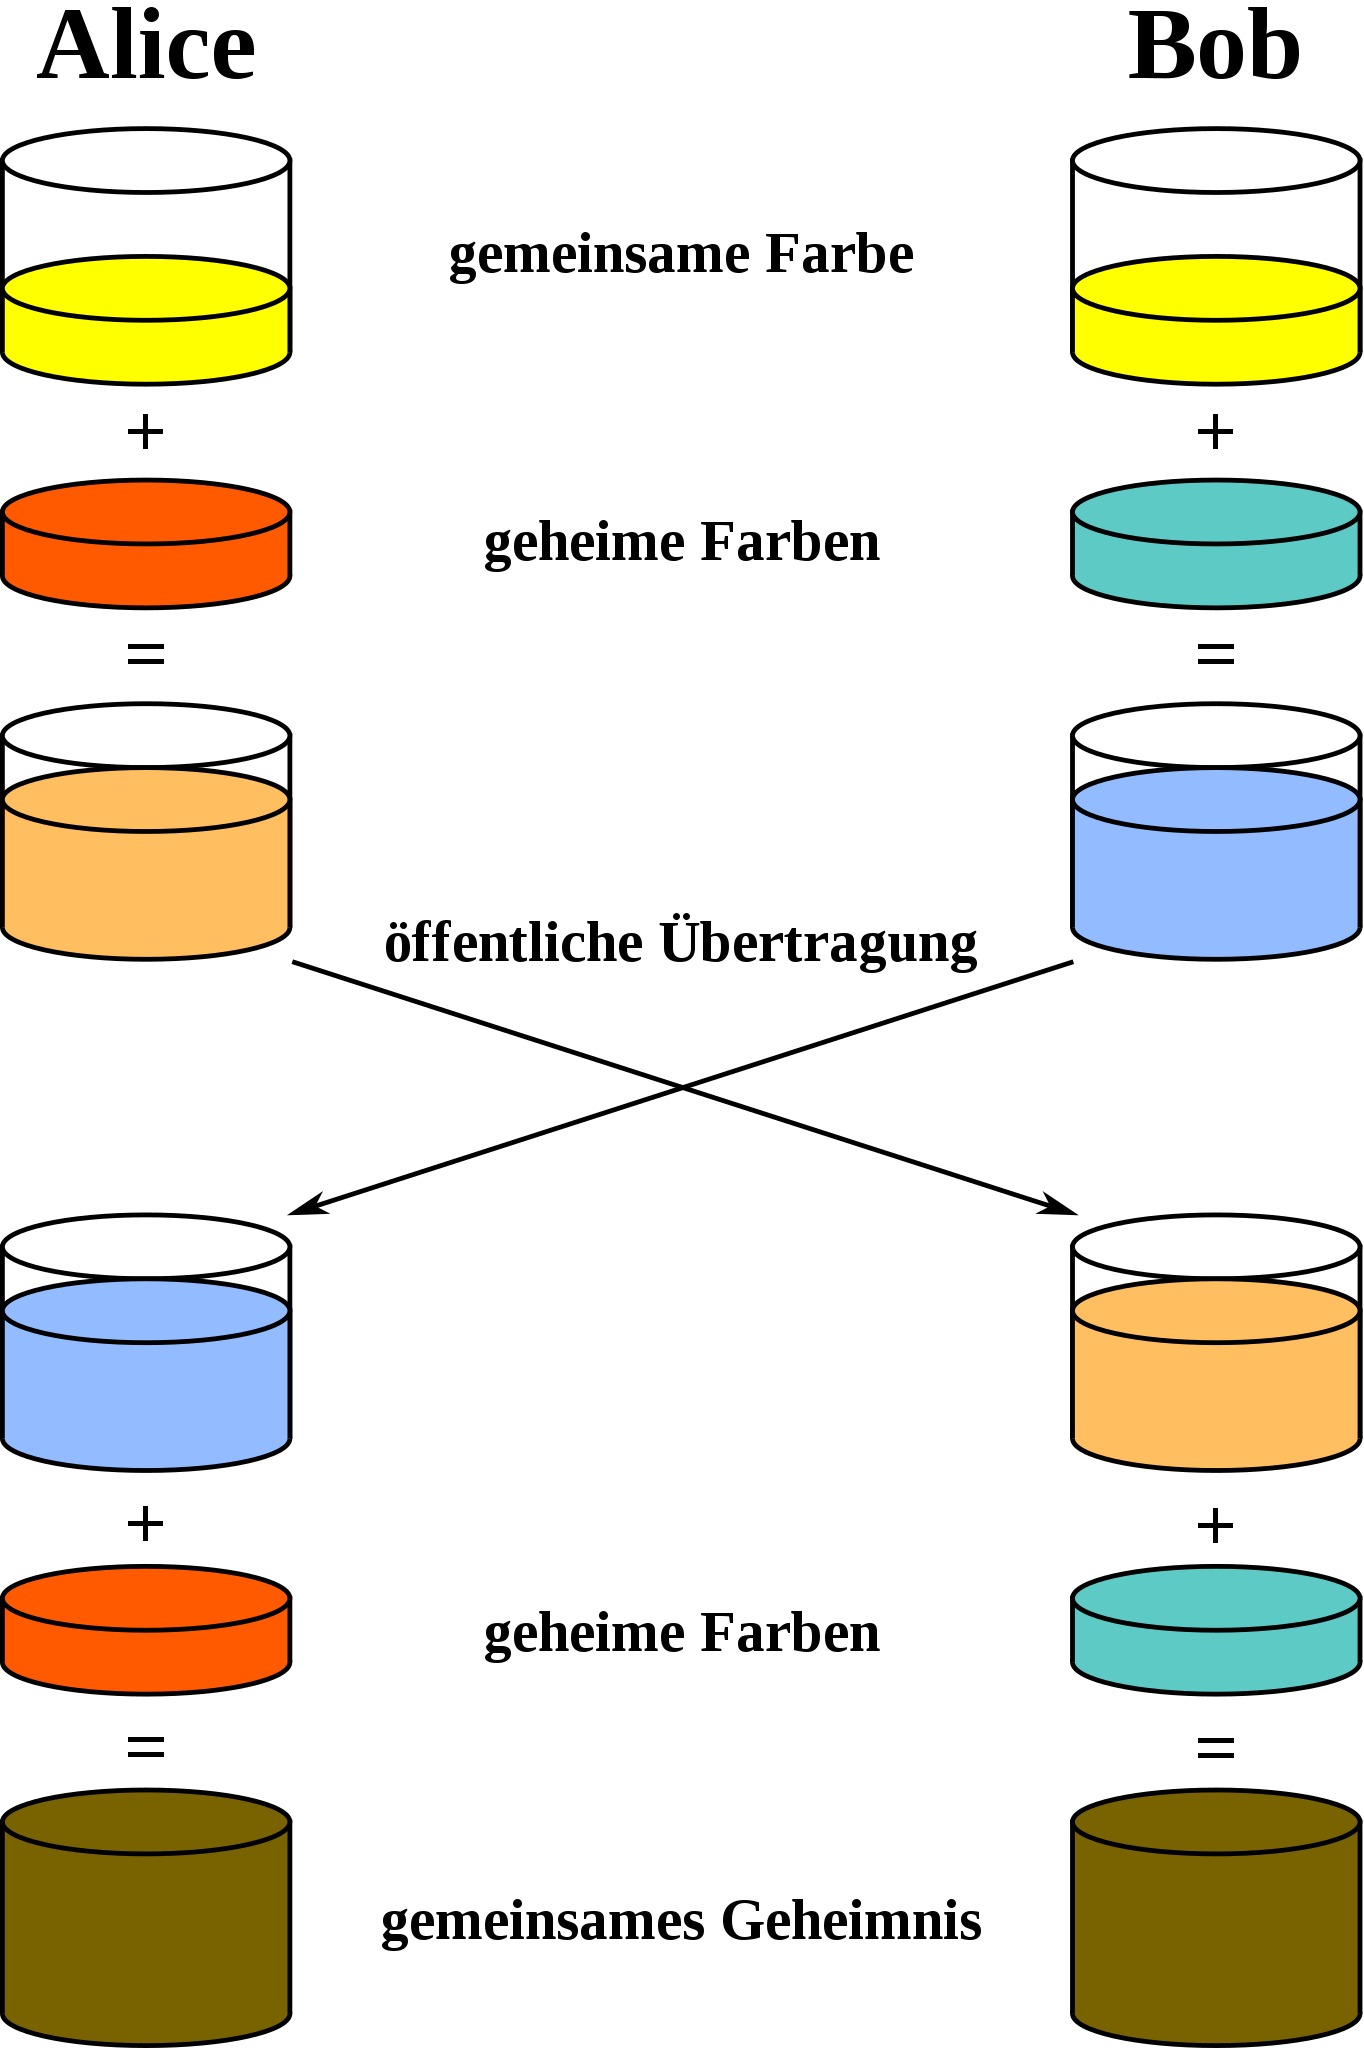
\includegraphics[scale=0.15]{dhm_schluesselvereinbarung_farben}
	\caption{Das gemeinsame Geheimnis (braune Farbe in der letzten Zeile) stellt den gemeinsamen geheimen Schlüssel von Alice und Bob dar.}
	\label{dhm-schluesselvereinbarung-farben}
\end{figure}

Nun gilt es, das Prinzip der Farbmischung auf mathematische Operationen zu übertragen. Diffie und Hellman kamen dazu auf die geniale Idee, das \textbf{modulare Rechnen mit Primzahlen} zu verwenden. Die beiden Forscher fanden heraus, dass die Rechnung mit \textbf{Potenzen und Modulo} einfach ist und es ermöglicht einen gemeinsamen Schlüssel zu vereinbaren. Gleichzeitig stellten Sie fest, dass der \textbf{diskrete Logarithmus} unter gewissen Bedingungen in keiner vernünftigen Zeit lösbar ist. Dadurch kann ein Angriff von Eve verhindert werden. Diese beiden Eigenschaften nutzen Sie aus für die Erfindung eines Protokolls zur Schlüsselvereinbarung. Die damit verbundenen Erkenntnisse läuteten zudem eine neue Ära in der Kryptologie ein.

\begin{hinweis}
	Diffie, Hellman und Merkle präsentierten die Verwendung der Potenzen in Kombination mit der Modulorechnung \textbf{vor} der Veröffentlichung des Protokolls \texttt{MASSEY-OMURA-SCHEMA}. Massey und Omura nutzten die Veröffentlichung von Diffie, Hellman und Merkle und erstellten ein alternatives Protokoll für die Schlüsselfestlegung.
\end{hinweis}

Wir zeigen erst ein Beispiel für die Schlüsselvereinbarung und notieren dann das Protokoll.

\begin{example}

Alice und Bob einigen sich auf die Zahlen $g = 2$ und $p = 19$. Diese Zahlen sind öffentlich bekannt. Wie in den vorherigen Protokollen sind $\text{key}_A$ bzw. $\text{key}_B$ geheim und nur in Besitz von Alice bzw. Bob.

\begin{figure}[htb]
\begin{tikzpicture}
\node[inner sep=0pt] (eve) at (0,0) {
\includegraphics[scale=0.25]{eve_tiny}};
\node[text width=2cm, align=center] (pangreifer) at (0, 1) {Eve};
\node[inner sep=0pt] (alice) at (-5,0) {
\includegraphics[scale=0.25]{alice_tiny}};
\node[text width=2cm, align=center] (sender) at (-5, 1) {Alice};
\node[inner sep=0pt] (bob) at (4,0) {
\includegraphics[scale=0.25]{bob_tiny}};
\node[text width=2cm, align=center] (empfaenger) at (4, 1) {Bob};

\node[text width=1cm, align=center, fill=black!25] (step1) at (-7, -1.25) {\Huge 1};
\node[text width=4cm, anchor=west] (step1ActionAlice) at (-6, -1.25) {$\text{key}_A = 3$};
\node[text width=3cm, anchor=west] (step1ActionBob) at (3, -1.25) {$\text{key}_B = 4$};


\node[text width=1cm, align=center, fill=black!25] (step2) at (-7, -2.5) {\Huge 2};
\node[text width=3cm, anchor=west] (step2ActionAlice) at (-6, -2.5) {%
$\begin{aligned}
     \text{msg}_A & = g^{\text{key}_A} \bmod p \\ 
     & = 2^{3} \bmod 19 = 8
  \end{aligned}$
};
\node[text width=2cm, anchor=west] (step2ActionBob) at (3, -2.5) {%
$\begin{aligned}
     \text{msg}_B & = g^{\text{key}_B} \bmod p\\ 
     & = 2^{4} \bmod 19 = 16
  \end{aligned}$
};

\node[text width=1cm, align=center, fill=black!25] (step3) at (-7, -4) {\Huge 3};
\node[text width=3cm, anchor=west] (step3ActionAlice) at (-6, -4) {%
$\begin{aligned}
     \text{key}_S & = (\text{msg}_B)^{\text{key}_A} \bmod p \\ 
     & = 16^{3} \bmod 19 = 11
  \end{aligned}$
};
\node[text width=3cm, anchor=west] (step3ActionBob) at (3, -4) {%
$\begin{aligned}
     \text{key}_S & = (\text{msg}_A)^{\text{key}_B} \bmod p \\ 
     & = 8^{4} \bmod 19 = 11
  \end{aligned}$
};

\draw[-latex, very thick] ([xshift=20pt]step2ActionAlice.east) -- ([yshift=10pt]step3ActionBob.west) node[above, near start, sloped] {$\text{msg}_A = 8$};
\draw[-latex, very thick] (step2ActionBob.west) -- ([xshift=25pt]step3ActionAlice.east) node[above, near start, sloped] {$\text{msg}_B = 16$};

\end{tikzpicture}
\caption{Eve sieht nur die beiden Nachrichten $\text{msg}_A$ und $\text{msg}_B$ sowie die Zahlen $g$ und $p$.}
\label{figure-schluesselvereinbarung-dhm-example}
\end{figure}

Nach dem dritten Schritt erhalten beide den gemeinsamen geheimen Schlüssel $\text{key}_S = 11$.

\end{example}

Das Beispiel zeigt, dass sowohl Alice als auch Bob den gleichen gemeinsamen geheimen Schlüssel berechnen. Ist er jedoch wirklich geheim? Kann Eve mit bekannten Nachrichten und Zahlen vielleicht auf den gemeinsamen geheimen Schlüssel schliessen? Wie bereits beim Protokoll \texttt{MASSEY-OMURA-SCHEMA} muss der Kryptoanalytiker das Diskrete-Logarithmus-Problem lösen. Für das Beispiel von oben muss Eve folgende Gleichungen lösen:
\begin{align*}
	2^{\text{key}_A} \bmod 11 & = 8 \\
	2^{\text{key}_B} \bmod 11 & = 16
\end{align*}
Für kleine Zahlen kann Eve durch Ausprobieren die Zahlen erraten. Wählt man die Zahlen für $g$ und $p$ jedoch korrekt (z.B. $p$ muss eine grosse Primzahl sein), dann ist (aus der heutigen Sicht) das Ermitteln von $\text{key}_A$ bzw. $\text{key}_B$ ein schwieriges Problem und in keiner vernünftigen Zeit lösbar.

\subsection{Das Schlüsselvereinbarungsprotokoll \texttt{DIFFIE-HELLMAN-MERKLE}}

Wir definieren nun das exakte Schlüsselverteilungsprotokoll.

\begin{definition}[Protokoll \texttt{DIFFIE-HELLMAN-MERKLE}]
\textbf{Ziel}: Alice und Bob besitzen einen gemeinsamen geheimen Schlüssel (eine natürliche Zahl). \\ \textbf{Vorbereitung}: Alice und Bob einigen sich auf eine grosse Primzahl $p$. Diese Primzahl muss nicht geheim gehalten werden. Alle Zahlen sind nun aus der Menge $\mathbb{Z}_{p}^*$ zu wählen. Nachdem $p$ gewählt wurde, einigen sich Alice und Bob auf eine weitere Zahl $g$ aus $\mathbb{Z}_{p}^*$.


\begin{enumerate}
	\item Alice wählt zufällig eine Zahl aus $\mathbb{Z}_{p}^*$ und hält diese geheim, d.h. $\text{key}_A \in \mathbb{Z}_{p}^*$. Bob wählt ebenfalls eine zufällige Zahl aus $\mathbb{Z}_{p}^*$ und hält diese auch geheim, d.h. $\text{key}_B \in \mathbb{Z}_{p}^*$.
	\item Alice berechnet nun $\text{msg}_A = g^{\text{key}_A} \bmod p$ und schickt $\text{msg}_A$ an Bob. Bob berechnet $\text{msg}_B = g^{\text{key}_B} \bmod p$ und schickt $\text{msg}_B$ an Alice.
	\item Alice erhält $\text{msg}_B$ und berechnet $\text{key}_S = (\text{msg}_B)^{\text{key}_A} \bmod p$. Bob erhält $\text{msg}_A$ und berechnet $\text{key}_S = (\text{msg}_A)^{\text{key}_B} \bmod p$.
\end{enumerate}

Beide berechnen den gemeinsamen geheimen Schlüssel $\text{key}_S$.

\end{definition}

Bei genauer Betrachtung des Protokolls, stellt man fest, dass keine Partei bei der Schlüsselvereinbarung bevorzugt wird. Ausserdem wählen Alice und Bob ihre geheimen Schlüssel gleichzeitig. Auch das Berechnen des gemeinsamen geheimen Schlüssel kann parallel erfolgen.

\subsection{Aufgaben}

\begin{enumerate}
	\item Skizzieren Sie das Protokoll \texttt{DIFFIE-HELLMAN-MERKLE} für die Werte $p = 17$, $g = 3$, $\text{key}_A = 6$ und $\text{key}_B = 4$. Notieren Sie auch die Rechenschritte von Alice und Bob.
	\item Wie lautet der gemeinsame geheime Schlüssel, wenn Alice und Bob das Schlüsselvereinbarungsprotokoll \texttt{DIFFIE-HELLMAN-MERKLE} mit $p = 27\,803$, $g = 5$, $\text{key}_A = 21\,131$ und $\text{key}_B = 17\,555$ anwenden.
	\item Alice und Bob erhalten mit dem Protokoll \texttt{DIFFIE-HELLMAN-MERKLE} den gemeinsamen geheimen Schlüssel $\text{key}_S = 11\,134$. Sie möchten nun zur Kommunikation ein symmetrisches Kryptosystem verwenden.
	\begin{enumerate}
		\item Wie können Alice und Bob den gemeinsamen geheimen Schlüssel $\text{key}_S$ als Schlüssel für \texttt{VIGENÈRE} benutzen?
		\item Wie können Alice und Bob den gemeinsamen geheimen Schlüssel $\text{key}_S$ als Schlüssel für \texttt{ONE-TIME-PAD} benutzen?
	\end{enumerate}
\end{enumerate}

\subsection{Korrektheit des Protokolls}

Wir müssen nun zeigen, dass das Protokoll \texttt{DIFFIE-HELLMAN-MERKLE} korrekt arbeitet. Wir zeigen, dass Alice und Bob wirklich den gleichen geheimen Schlüssel berechnen. Alice berechnet:
\begin{align*}
	\text{key}_S	& = (\text{msg}_B)^{\text{key}_A} \bmod p \\
					& = (g^{\text{key}_B} \bmod p)^{\text{key}_A} \bmod p \\
					\shortintertext{\centering $\bmod p$ muss nur einmal berechnet werden:}
					& = (g^{\text{key}_B})^{\text{key}_A} \bmod p \\
										\shortintertext{\centering Potenzgesetze:}
					& = g^{\text{key}_B \cdot \text{key}_A} \bmod p
\end{align*}
Auf der anderen Seite berechnet Bob:
\begin{align*}
	\text{key}_S	& = (\text{msg}_A)^{\text{key}_B} \bmod p \\
					& = (g^{\text{key}_A} \bmod p)^{\text{key}_B} \bmod p \\
					\shortintertext{\centering $\bmod p$ muss nur einmal berechnet werden:}
					& = (g^{\text{key}_A})^{\text{key}_B} \bmod p \\
										\shortintertext{\centering Potenzgesetze:}
					& = g^{\text{key}_A \cdot \text{key}_B} \bmod p
\end{align*}
Da die modulare Multiplikation kommutativ ist, gilt $\text{key}_S = g^{\text{key}_A \cdot \text{key}_B} \bmod p = g^{\text{key}_B \cdot \text{key}_A} \bmod p$. Alice und Bob berechnen also tatsächlich immer den gleichen geheimen Schlüssel. 

\subsection{Sicherheit des Protokolls}

Ist das Protokoll sicher? Eve erhält die Zahlen $p$ und $g$ sowie die Nachrichten $\text{msg}_A$ und $\text{msg}_B$. Falls Eve aus den Gleichungen
\begin{align*}
	g^{\text{key}_A} \bmod p & = \text{msg}_A \\
	g^{\text{key}_B} \bmod p & = \text{msg}_B
\end{align*}
die beiden geheimen Zahlen $\text{key}_A$ und $\text{key}_B$ bestimmen kann, dann ist es mit $\text{key}_S = g^{\text{key}_A \cdot \text{key}_B} \bmod p$ möglich den gemeinsamen geheimen Schlüssel zu berechnen. Es ist aber ausserordentlich schwer, von $g^{\text{key}_A} \bmod p = \text{msg}_A$ auf $\text{key}_A$ zu schliessen. Auch beim Protokoll \texttt{DIFFIE-HELLMAN-MERKLE} muss Eve das Diskrete-Logarithmus-Problem lösen. Wie bereits beim \texttt{MASSEY-OMURA-SCHEMA} erwähnt, gibt es aus der heutigen Sicht kein Verfahren, um das Problem in vernünftiger Zeit zu lösen. Man könnte sich noch vorstellen, dass Eve nicht notwendigerweise die geheimen Zahlen $\text{key}_A$ und $\text{key}_B$ berechnen muss. Vielleicht ist es möglich aus den beiden Nachrichten $\text{msg}_A$ und $\text{msg}_B$ den gemeinsamen geheimen Schlüssel $\text{key}_S$ direkt zu berechnen. Leider ist es bisher keiner Person gelungen, solch eine Berechnung zu finden. Auch gibt es bisher keinen Beweis dafür, dass das Knacken des Protokolls \texttt{DIFFIE-HELLMAN-MERKLE} gleichwertig ist zum Berechnen des diskreten Logarithmus.

\begin{important}
	Das Protokoll \texttt{DIFFIE-HELLMAN-MERKLE} ist nur dann sicher, wenn $p$ und $g$ korrekt gewählt werden. $p$ muss eine grosse Primzahl sein und $g$ ein Generator für $\mathbb{Z}_{p}^*$ mit der modularen Multiplikation $\odot_{p}$. Einen Generator zu finden, ist keine einfache Aufgabe. Es gibt jedoch Tricks. Man kann eine sogenannte \say{sichere Primzahl} wählen. Dies ist eine Primzahl $p$ für die gilt: $p = 2 \cdot q + 1$ für eine Primzahl $q$. Dann gibt es genügend Generatoren und man kann mit einem randomisierten Algorithmus recht effizient einen Generator finden. Wählt man für $g$ keinen Generator, dann muss man für das Lösen des diskreten Logarithmus, das heisst $g^a = x \bmod p$ nicht alle Zahlen für $a$ ausprobieren. Die Brute-Force-Methode wäre dann möglich.
\end{important}

\subsection{Aufgaben}

\begin{enumerate}
	\item Es sind $p = 11$, $g = 4$ und $\text{msg}_A = 3$ bekannt. Versuchen Sie $\text{key}_A$ zu bestimmen.
	\item Versuchen Sie das Schlüsselvereinbarungsprotokoll \texttt{DIFFIE-HELLMAN-MERKLE} zu knacken, indem Sie für die gegebenen Werte $p$, $g$, $\text{msg}_A$ und $\text{msg}_B$ jeweils die geheimen Zahlen $\text{key}_A$ und $\text{key}_B$ berechnen und daraus dann den vereinbarten Schlüssel $\text{key}_S$.
	\begin{enumerate}
		\item $p = 5$, $g = 3$, $\text{msg}_A = 4$ und $\text{msg}_B = 2$
		\item $p = 13$, $g = 2$, $\text{msg}_A = 6$ und $\text{msg}_B = 11$
		\item $p = 7$, $g = 2$, $\text{msg}_A = 2$ und $\text{msg}_B = 4$
	\end{enumerate}
	\item Angenommen, Sie kennen die Gleichung $7^x \bmod 31 = 10$. Bestimmen Sie $x$.
	\item Versuchen Sie das Protokoll \texttt{DIFFIE-HELLMAN-MERKLE} zu knacken, indem Sie aus den Werten $p = 29$, $g = 11$, $\text{msg}_A = 7$ und $\text{msg}_B = 15$ den Schlüssel $\text{key}_S$ bestimmen.
\end{enumerate}

\section{\texttt{DIFFIE-HELLMAN-MERKLE} versus \texttt{MASSEY-OMURA-SCHEMA}}

Beide Protokolle ermöglichen die Schlüsselfestlegung. Wir stellen hier die beiden Verfahren nun gegenüber.

% Vor und Nachteile bei Diffie vs Massey
% https://faubox.rrze.uni-erlangen.de/dl/fiS4uFvUTecsHKgp5yttK3Ae/ki_dlogan.pdf?inline

\begin{table}[htb]
\centering
\begin{tabular}{|p{3.5cm}|p{5cm}|p{5.5cm}|}
\hline
\textbf{Kriterium} & \texttt{MASSEY-OMURA-SCHEMA} & \texttt{DIFFIE-HELLMAN-MERKLE} \\ \hline
\textbf{Anzahl Nachrichten} & 3 & 2 \\ \hline
\textbf{Nicht geheime Zahlen} & Primzahl $p$ & Primzahl $p$ und Generator $g$ \\ \hline
\textbf{Sicherheit} & Falls $p$ gross genug gewählt wird, ist das Verfahren gegen passive Angreifer sicher.                                                                               & Falls $p$ gross genug gewählt wird und $g$ ein Generator ist, dann ist das Verfahren gegen passive Angreifer sicher. \\ \hline
\textbf{Verständlichkeit} & Modulares Potenzieren ist relativ einfach anzuwenden. Der modulare Kehrwert benötigt ein tieferes Verständnis der modularen Arithmetik und ist von Hand mühsam zu berechnen. & Es wird nur das modulare Potenzieren benötigt. Dies ist relativ einfach anzuwenden. \\ \hline
\textbf{Einsatz in der Praxis} & Mir ist nicht bekannt, ob das Protokoll in der Praxis eingesetzt wird. & Standard in der modernen Kryptographie. Einsatzgebiet: Verschlüsselungsprotokolle im Internet (\ac{TLS}) \\ \hline
\end{tabular}
\end{table}

\section{Sicherheit der Protokolle bei aktiven Angreifern}

Alle bisherigen Überlegungen sind von Eve als passive Angreiferin ausgegangen. Ein passiver Kryptoanalytiker kann lauschen und somit Nachrichten kopieren. Er darf sich jedoch nicht in das Kommunikationsprotokoll oder Kryptosystem einmischen. Wir wollen nun die Rolle von Eve anpassen. Aus Eve wird nun eine \textbf{aktive Angreiferin} die wir Mallory\footnote{Der Name Mallory wird gerne deshalb benutzt, da eine Ähnlichkeit zu malicious besteht (dt. böswillig, hinterhältig, heimtückisch).} nennen. Nun darf Mallory in die Kommunikation eingreifen. Dies kann zum Beispiel durch das \textbf{Abfangen} von Nachrichten oder die \textbf{Manipulation} von Nachrichten geschehen. Ist unter diesen Voraussetzungen das Protokoll \texttt{DIFFIE-HELLMAN-MERKLE} sicher? Ohne weitere Vorkehrungen von Alice und Bob kann Mallory wie in \autoref{figure-schluesselvereinbarung-dhm-example-man-in-the-middle} in das Protokoll eingreifen.

\begin{figure}[htb]
\begin{tikzpicture}
\node[inner sep=0pt] (mallory) at (1,0) {
\includegraphics[scale=0.25]{mallory_tiny}};
\node[text width=2cm, align=center] (aangreifer) at (1, 1) {Mallory};
\node[inner sep=0pt] (alice) at (-5,0) {
\includegraphics[scale=0.25]{alice_tiny}};
\node[text width=2cm, align=center] (sender) at (-5, 1) {Alice};
\node[inner sep=0pt] (bob) at (5,0) {
\includegraphics[scale=0.25]{bob_tiny}};
\node[text width=2cm, align=center] (empfaenger) at (5, 1) {Bob};

\node[text width=1cm, align=center, fill=black!25] (step1) at (-7, -1.25) {\Huge 1};
\node[text width=4cm, anchor=west] (step1ActionAlice) at (-6, -1.25) {$\text{key}_A = 3$};
\node[text width=3cm] (step1ActionBob) at (6, -1.25) {$\text{key}_B = 4$};
\node[text width=3cm, anchor=west] (step1ActionMallory) at (0, -1.25) {$\text{key}_M = 5$};


\node[text width=1cm, align=center, fill=black!25] (step2) at (-7, -2.5) {\Huge 2};
\node[text width=3cm, anchor=west] (step2ActionAlice) at (-6, -2.5) {%
$\begin{aligned}
     \text{msg}_A & = g^{\text{key}_A} \bmod p \\ 
     & = 2^{3} \bmod 19 = 8
  \end{aligned}$
};
\node[text width=2cm, anchor=west] (step2ActionMallory) at (0, -2.5) {%
$\begin{aligned}
     \text{msg}_M & = g^{\text{key}_M} \bmod p\\ 
     & = 2^{5} \bmod 19 = 13
  \end{aligned}$
};

\node[text width=1cm, align=center, fill=black!25] (step3) at (-7, -4) {\Huge 3};
\node[text width=3cm, anchor=west] (step3ActionAlice) at (-6, -4) {%
$\begin{aligned}
     \text{key}_S & = (\text{msg}_M)^{\text{key}_A} \bmod p \\ 
     & = 13^{3} \bmod 19 = 12
  \end{aligned}$
};
\node[text width=3cm, anchor=west] (step3ActionMallory) at (0, -4) {%
$\begin{aligned}
     \text{key}_S & = (\text{msg}_A)^{\text{key}_M} \bmod p \\ 
     & = 8^{5} \bmod 19 = 12
  \end{aligned}$
};

\draw[-latex, very thick] ([xshift=15pt, yshift=-10pt]step2ActionAlice.east) -- ([yshift=10pt]step3ActionMallory.west) node[above, near start, sloped] {$\text{msg}_A = 8$};
\draw[-latex, very thick] ([xshift=25pt, yshift=-15pt]step2ActionMallory.west) -- ([xshift=25pt, yshift=5pt]step3ActionAlice.east) node[above, near start, sloped] {$\text{msg}_M = 13$};

\end{tikzpicture}
\caption{Mallory greift aktiv in das Protokoll ein und fängt die Nachricht von Alice ab.}
\label{figure-schluesselvereinbarung-dhm-example-man-in-the-middle}
\end{figure}

Mallory kann zwar nicht den gemeinsamen Schlüssel von Alice und Bob berechnen, sie kann sich jedoch zwischen die beiden Parteien schalten. Sie nimmt quasi die Rolle von Bob ein und macht mit Alice einen Schlüssel ab. Die ahnungslose Alice empfängt die Nachricht von Mallory und berechnet den gemeinsamen geheimen Schlüssel. Auch Mallory kann den gemeinsamen geheimen Schlüssel berechnen, da sie die Nachricht von Alice abfängt. Nun kann Mallory alle Nachrichten, die Alice verschlüsselt, abfangen und entschlüsseln, da sie den gleichen geheimen Schlüssel wie Alice besitzt. Auch wenn wir in \autoref{figure-schluesselvereinbarung-dhm-example-man-in-the-middle} die Nachricht mit $\text{msg}_M$ bezeichnen, merken Alice und Bob unter Umständen nicht, dass Mallory in das Protokoll eingegriffen hat. Alice erhält schliesslich eine Nachricht, wenn auch nicht vom korrekten Partner. Bob weiss möglicherweise gar nicht, dass ihm etwas entgangen ist.

%https://www.bsi.bund.de/SharedDocs/Glossareintraege/DE/M/Man-In-The-Middle-Angriff.html

\begin{definition}[Man-in-the-Middle-Angriff]
	Ziel bei einem Man-in-the-Middle-Angriff ist es, sich unbemerkt in eine Kommunikation zwischen zwei oder mehr Partnern einzuschleichen, beispielsweise um Informationen mitzulesen oder zu manipulieren. Hierbei begibt sich die Angreiferin (Mallory) \say{in die Mitte} der Kommunikation, indem sie sich gegenüber dem Sender (Alice) als Empfänger (Bob) und gegenüber dem Empfänger (Bob) als Sender (Alice) ausgibt. Zuerst leitet die Angreiferin (Mallory) eine Nachricht des Senders zu sich um. Im nächsten Schritt schickt die Angreiferin eine Nachricht zu dem eigentlichen Empfänger. Wenn ihr das gelingt, kann die Angreiferin unter Umständen alle Informationen, die der Sender an den vermeintlichen Empfänger sendet, einsehen oder manipulieren, bevor Mallory sie an den richtigen Empfänger weiterleitet. Auf die Antworten des Empfängers kann die Angreiferin wiederum ebenfalls zugreifen.
\end{definition}

Alice muss sich also sicher sein, dass sie mit dem \say{echten} Bob kommuniziert. Bob muss sich sicher sein, dass er mit der \say{echten} Alice kommuniziert. Eine Kryptoanalytikerin darf sich nicht in die Kommunikation einschalten und sich als Alice oder Bob ausgeben. Wie können Alice und Bob sicher sein, dass sie mit der richtigen Person kommunizieren? Dafür muss man die Nachrichten mit einer digitalen Unterschrift versehen. Dies besprechen wir in einem separaten Kapitel.

\subsection{Aufgaben}

\begin{enumerate}
	\item Ist das Protokoll \texttt{MASSEY-OMURA-SCHEMA} gegen einen Man-in-the-Middle-Angriff geschützt? Begründen Sie Ihre Antwort mit einem Beispiel.
	\item Erweitern Sie den Man-in-the-Middle-Angriff aus \autoref{figure-schluesselvereinbarung-dhm-example-man-in-the-middle}. Alle Nachrichten von Alice an Bob sollen über Mallory verlaufen. Mallory soll auch alle Nachrichten von Bob an Alice erhalten. Wie kann Mallory sowohl die Nachrichten von Alice als auch die Nachrichten von Bob entschlüsseln?
\end{enumerate}

Diffie, Hellman und Merkle erkannten das Potenzial des diskreten Logarithmus und nutzen dies für die erste Entwicklung eines Schlüsselfestlegungsprotokolls. Dabei hatten Sie nicht das Ziel ein Protokoll mit perfekter Sicherheit zu erstellen, sondern eine \say{neue} Art der Sicherheit zu etablieren.

\begin{definition}[Modernes Sicherheitsverständnis]
	Ein Kryptosystem oder kryptografisches Kommunikationsprotokoll ist sicher, wenn die Kryptoanalyse so viel Zeit und Arbeit in Anspruch nimmt, dass die Kryptoanalyse in der Praxis nicht ausgeführt werden kann. Dabei darf die Art der Verschlüsselung und Entschlüsselung bekannt sein (Prinzip von Kerkhoff).
\end{definition}

Mit den Erkenntnissen von Diffie, Hellman und Merkle entstand ein völlig neuer Zweig der Kryptographie. Daraus entstanden moderne Kryptosysteme, welche zum Beispiel für elektronische Signaturen im Internet grossflächig eingesetzt werden. Wir schauen uns deshalb das Schlüsselfestlegungsprotokoll von Diffie, Hellman und Merkle an. Die damit verbundenen Konzepte wurden im Protokoll \texttt{MASSEY-OMURA-SCHEMA} aufgegriffen und eingesetzt. Das Protokoll \texttt{DIFFIE-HELLMAN-MERKLE} ist eine Alternative zum Protokoll \texttt{MASSEY-OMURA-SCHEMA} für die Schlüsselfestlegung. Es ist sogar so verbreitet, dass es gewissermassen den Standard für die Schlüsselfestlegung darstellt.